% Preprint template for the BIND Lightcone Suite drafts.
% Copy to papers/<id>/main.tex and fill. Keep the preamble minimal —
% it must compile with a plain TeX Live install (pdflatex + bibtex).
\documentclass[11pt]{article}
\usepackage[margin=1in]{geometry}
\usepackage{graphicx}
\usepackage{amsmath,amssymb}
\usepackage[round,authoryear]{natbib}
\usepackage[colorlinks=true,linkcolor=blue,citecolor=blue,urlcolor=blue]{hyperref}
\usepackage{xcolor}

% ---- shared macros (use these; the coherence pass checks for them) ----
\newcommand{\bind}{\textsc{bind}}
\newcommand{\Sell}{S(\ell)}                    % WL suppression S(l) = Cl_baryon/Cl_DMO
\newcommand{\kappay}{\kappa\times y}
\newcommand{\fgas}{f_{\rm gas}}
\newcommand{\Msun}{{\rm M}_\odot}
\newcommand{\Mhalo}{M_{200c}}
\newcommand{\zs}{z_{\rm s}}
\newcommand{\sez}{S(\ell, z_{\rm s})}
\newcommand{\todo}[1]{\textcolor{red}{[TODO: #1]}}

% ---- paper-specific shorthand ----
\newcommand{\faniso}{f_{\rm aniso}}
\newcommand{\ftri}{f_{\rm tri}}
\newcommand{\fmono}{f_{\rm mono}}
\newcommand{\kbind}{\kappa_{\rm bind}}
\newcommand{\ksph}{\kappa_{\rm sph}}
\newcommand{\kdmo}{\kappa_{\rm dmo}}

\title{The BIND Lightcone Suite V: How Anisotropic Is the Baryonic
Suppression of Weak Lensing?}
\author{%
  Max E.\ Lee$^{1,2}$ \todo{author list to be finalized}\\[2pt]
  \small $^1$Department of Astronomy, Columbia University, New York, NY, USA\\
  \small $^2$Center for Computational Astrophysics, Flatiron Institute, New York, NY, USA
}
\date{Draft: \today}

\begin{document}
\maketitle

\begin{abstract}
Baryonification methods (BCMs) correct dark-matter-only (DMO) simulations
for baryonic physics by displacing each halo's mass \emph{radially}, which
by construction discards any angular structure in the resulting correction.
Whether that discarded structure matters for weak lensing (WL) has not
previously been measured at the field level, because doing so requires a
generative model that paints hydrodynamic-quality baryon fields onto DMO
halos one-by-one so that a literal spherical counterfactual can be built
and differenced against the full field. We use \bind{}, a conditional
flow-matching emulator trained on the CAMELS-IllustrisTNG suite, to
construct exactly this counterfactual: a mass-exact, per-halo radial
``BCM-warp'' of the painted field that conserves each halo's monopole mass
profile while removing only its angular ($m\!\geq\!2$) structure. On the
fiducial-feedback lightcone ($\zs=1$), the fraction of the convergence
power-spectrum suppression that survives this symmetrization is
scale-dependent: $\faniso\approx0.45$ at $\ell=3\times10^3$, falling to
$0.24$ at $\ell=10^4$ and to $\approx0$ by $\ell=2\times10^4$.\ % src: dossier Result/corrected-f_aniso; examples/bcm_warp_comparison.py, WORKLOG:1144
This corrects an earlier, cruder estimate that forced the correction
\emph{itself} to be azimuthally symmetric and thereby credited a real BCM
with zero triaxiality response; that estimate returns a roughly
scale-flat $\fmono\approx0.5$, which we show is dominated at small scales
by halo triaxiality a real BCM already reproduces, not by missed feedback
physics.\ % src: dossier HEADLINE CORRECTION; WORKLOG:1144-1157
Even so, the corrected signal is non-negligible in amplitude at
$\ell\lesssim10^4$ \todo{a formal bootstrap/significance test for the
corrected \texttt{bcm\_warp}-control $\faniso$ has not yet been computed
in our source material; the only significance number available
($z=52.3\sigma$, \S\ref{sec:old}) belongs to the superseded \texttt{mono}
control, not this one} and its existence at any scale means
spherically-symmetric BCMs must over-eject
gas radially to fit the two-point function, biasing the recovered gas
profile in a way that plausibly explains why such models fail
non-Gaussian statistics. We identify AGN kinetic-mode and stellar-wind
feedback parameters as the strongest controls of the (upper-bound) angular
signal from 60 one-at-a-time TNG feedback variations.\ % src: dossier Result/feedback-channels; WORKLOG:1217-1232
This is a first, preliminary field-level measurement at fixed cosmology
and fiducial feedback; we flag explicitly which parts of the argument
still rest on the superseded control.
\end{abstract}

\section{Introduction}\label{sec:intro}

Hydrodynamical simulations are too expensive to run at the volumes and
parameter-space coverage required for stage-IV weak-lensing (WL)
cosmology, so baryonic effects on the matter power spectrum are instead
modeled by \emph{baryonification} -- post-hoc, analytic corrections
applied to cheap DMO simulations \citep{schneider_teyssier2015,
arico2020, mead2021}. Every widely used baryonification model shares one
structural assumption: gas and stars are redistributed \emph{radially}
within each halo, $r\to r'(r)$, so that the correction to the DMO density
field is by construction azimuthally symmetric around the halo center.
This assumption is convenient -- it reduces the correction to a
one-dimensional profile per halo, calibrated against the spherically
averaged gas fraction and pressure profiles of hydrodynamic simulations
-- but it is also, on its face, unphysical: feedback-driven gas ejection
follows the halo potential and large-scale environment, neither of which
is spherical, and the resulting anisotropy of real hydrodynamic
gas maps is well documented.\todo{find and cite a reference for
angular/quadrupole structure in hydrodynamic halo gas maps;
\citet{van_daalen2020} (arXiv:1906.00968), attached to this sentence in
an earlier draft, is a library of \emph{isotropic}, spherically-averaged
matter power spectra and an empirical suppression-amplitude-vs-$\fgas$
model -- it does not document angular gas-map anisotropy and does not
support this specific claim (verified against the full text).} What has
not been measured is how much of the WL observable itself -- the lensing
convergence power spectrum $C_\ell^{\kappa\kappa}$ that stage-IV surveys
use to marginalize over baryons -- is actually carried by this discarded
angular information, as opposed to the radial profile a spherical BCM
already captures.

Answering this at the field level requires a generative model that (i)
paints full hydrodynamic-quality baryon fields halo-by-halo, so that (ii)
one can build a faithful, per-halo spherical counterfactual of the
\emph{same} halos under the \emph{same} realization, and difference it
against the full field. \bind{} \citep[Paper I]{bindI} is exactly this
model: a conditional flow-matching emulator that paints
$[\mathrm{DM}_{\rm hydro},\,\mathrm{Gas},\,\mathrm{Stars}]$ maps onto DMO
halo cutouts, conditioned on the CAMELS-IllustrisTNG 35-parameter
cosmology+astrophysics vector. In this Letter we use the \bind{}
lightcone pipeline to build, for the first time, a literal radial
counterfactual of a full painted WL field and measure the fraction of the
convergence-power suppression that a spherically symmetric baryonification
model can never reproduce. We report this fraction as a function of scale
and identify the feedback channels that control it, while being explicit
that our fiducial control is a conservative, first field-level bound
rather than a final number (\S\ref{sec:discussion}).

\section{Methods}\label{sec:methods}

\subsection{Three fields, one set of halos}\label{sec:fields}

For every halo along the \bind{} lightcone we build three versions of the
same patch from the same DMO particles and the same painted realization:
a \texttt{dmo} field (no baryons), a \texttt{bind} field (the full BIND
composite, i.e.\ the hydrodynamic-quality painted map), and a spherical
control field that retains only the monopole of the \texttt{bind}
correction. Convergence maps $\kappa$ are then built by ray-tracing the
same lightcone through all three fields, so that cosmic variance,
projection/shape noise, and halo sampling cancel exactly in any
difference between them.

\subsection{The faithful radial-BCM-warp control}\label{sec:control}

The spherical control is the crux of the measurement, and we use two
versions of it here for a specific reason. An earlier implementation
(\texttt{azimuthal\_average\_patch}, ``mono'') simply azimuthally averages
the \emph{correction} $\Delta\Sigma=\Sigma_{\rm hydro}-\Sigma_{\rm dmo}$ in
each patch. This forces the correction itself to be circular, which is
\emph{not} what a real BCM does: an actual radial-push BCM (potential- or
mass-based displacement, in the spirit of e.g.\ \citealt{dai_feng_seljak2018})
moves mass along $r\to r'(r)$, so a triaxial halo's corrected surface
density remains triaxial even under a perfectly ``spherical'' baryon
model -- only the \emph{displacement law} is radial, not the resulting
map. The mono control therefore credits a real BCM with zero
triaxiality-tracing ability, which inflates the apparent missed
anisotropy by an amount set by the halo's intrinsic (DM) triaxiality
\citep{osato_triaxiality}.

Our primary, faithful control (\texttt{bcm\_warp\_patch}, ``sph'';
\texttt{mode="bcm\_warp"} in \texttt{bind.inference.spherical}) instead
pushes each DMO pixel radially so that $M_{\rm dmo}(<r)=M_{\rm
hydro}(<r')$ is satisfied mass-exactly (CIC-interpolated) about the
halo's own center. Because the push is purely radial, halo triaxiality
\emph{co-moves} with the mass flow exactly as it would under a real BCM;
only genuine \emph{angular} feedback structure -- azimuthal
non-uniformity in where gas is deposited or ejected, beyond what a radial
push of a triaxial halo already produces -- separates \texttt{sph} from
\texttt{bind}. \texttt{bcm\_warp\_patch} itself was verified at the time of
this control's introduction to conserve mass to $10^{-5}$, track the
hydro monopole, and preserve the DMO annular RMS, but that verification
is qualitative only in our source material.\ % src: WORKLOG:1172
\todo{a quantitative L2/correlation validation of \texttt{bcm\_warp\_patch}
specifically, of the kind reported below for \texttt{mono}, has not been
computed in the sources available to us.}
Separately -- and this is a validation of the crude \texttt{mono} control,
\emph{not} of \texttt{bcm\_warp\_patch} -- we stacked the monopole $c_0(r)$
of the BIND correction against the azimuthally-averaged \texttt{mono}
correction over cluster-mass halos: the two agree to an L2 relative
residual of $2.22\%$ with correlation $0.99998$, and the residual
$\texttt{bind}-\texttt{mono}$ is a pure $m\!\geq\!2$ field, with its own
monopole consistent with zero at the
$\mathrm{RMS}|c_0|/\mathrm{RMS}|c_2|=0.018$ level (i.e.\ the \texttt{mono}
control leaves the radial profile intact to $\sim\!2\%$ while removing
only the quadrupole-and-higher structure).\ % src: dossier Method/validation; wl_anisotropy_paper.ipynb cells 17-18, WORKLOG:1217
For the single most massive halo in the sample ($\log_{10}(\Mhalo/\Msun
h^{-1})=14.57$), the anisotropic component alone carries $97\%$ of the
correction's pixel RMS, illustrating how large the angular term can be
for an individual triaxial cluster.\ % src: dossier Method/validation; wl_anisotropy_paper.ipynb cell 17
This only shows that \texttt{mono} is a fair monopole-preserving
counterpart to \texttt{bind}; per the argument above, it does \emph{not}
by itself validate \texttt{bcm\_warp\_patch}, since the \texttt{mono}
residual conflates genuine feedback anisotropy with the
triaxiality-tracing term $\ftri$ that a faithful radial BCM would instead
capture (\S\ref{sec:headline}). Figure~\ref{fig:maps} shows one
realization of the resulting fields built with the \texttt{mono} control,
the only spherical control for which a rendered map exists in our source
material at the time of writing; the faithful \texttt{bcm\_warp}
control's field-level numbers instead appear in
Figure~\ref{fig:decomposition} (\S\ref{sec:headline}).\ % src: full-notebook
% grep of wl_anisotropy_paper.ipynb for "bcm_warp" returns zero hits; cell 20
% (the source of Figure~\ref{fig:maps}) imports azimuthal_average_patch, not
% bcm_warp_patch; only examples/bcm_warp_comparison.py (source of
% Figure~\ref{fig:decomposition}) actually uses bcm_warp_patch

\begin{figure}[t]
\centering
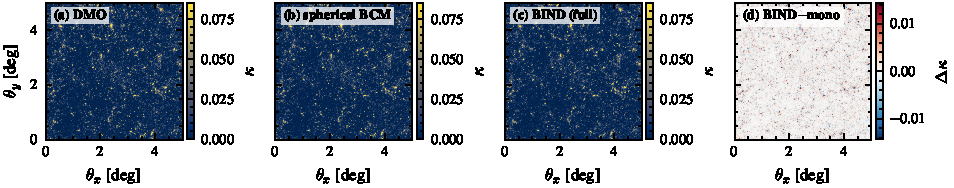
\includegraphics[width=\textwidth]{figs/fig01_maps.pdf}
\caption{Convergence maps built from the \emph{same} halos and the same
lightcone realization at $\zs=1$: DMO-only, the crude pure-spherical
\texttt{mono} control (panel label ``spherical BCM''), the full \bind{}
composite, and their difference $\kbind-\kappa_{\rm mono}$ (rightmost
panel). \emph{This figure uses the earlier, superseded \texttt{mono}
control (\S\ref{sec:control}), not the faithful \texttt{bcm\_warp}
control} -- no rendered \texttt{bcm\_warp} map exists in our source
material at the time of writing. The difference panel is therefore an
\emph{upper bound} on the pure angular signal: it also contains the
triaxiality-tracing term $\ftri$ that a faithful radial BCM would remove
(\S\ref{sec:headline}), not only the genuine feedback anisotropy
$\faniso$ -- but it is still visually concentrated on massive, triaxial
halos rather than spread uniformly across the field. % src: dossier
% FIGURES #2; wl_anisotropy_paper.ipynb cell 20; see \S\ref{sec:control} for
% the mono-vs-bcm\_warp attribution
}
\label{fig:maps}
\end{figure}

\subsection{Field statistic and the first-order mechanism}\label{sec:mechanism}

For any map statistic $X$ we define the total baryonic effect
$\Delta X_{\rm baryon}=X_{\rm bind}-X_{\rm dmo}$, the anisotropic
component $\Delta X_{\rm aniso}=X_{\rm bind}-X_{\rm sph}$, and the
anisotropic fraction $\faniso(X)=\Delta X_{\rm aniso}/\Delta X_{\rm
baryon}$. For the convergence power spectrum this admits an exact
decomposition,
\begin{equation}
\Delta P \equiv P_{\rm bind}-P_{\rm sph} = \underbrace{2\,{\rm Re}
\big\langle \mathcal{F}[\kdmo]^{*}\,\mathcal{F}[\kbind-\ksph]\big\rangle}
_{\text{cross, first order}} \;+\; \underbrace{\big\langle
|\mathcal{F}[\delta_{\rm bind}]|^2\big\rangle -
\big\langle|\mathcal{F}[\delta_{\rm sph}]|^2\big\rangle}
_{\text{auto, second order}},
\end{equation}
with $\delta\equiv\kappa-\kdmo$. The cross term is first order in the
angular correction because it is linear in $(\kbind-\ksph)$, weighted by
the (large) DMO field itself; the auto term is quadratic in the
(small) correction and can even have the ``wrong'' sign. Physically, the
cross term dominates when the angular correction is spatially aligned
with the halo's own DMO lensing signal -- expected, since feedback-driven
gas redistribution follows the halo potential, i.e.\ the same matter that
lenses. On the fiducial lightcone (8 paired realizations, $\zs=1$, band
$\ell\in[3\times10^3,2\times10^4]$) this identity closes to machine
precision and gives cross$/\Delta P\approx+1.39$ and
auto$/\Delta P\approx-0.39$ (rising to $\approx1.95/-0.95$ by
$\ell\sim1.8\times10^4$), confirming that the anisotropic suppression is
carried at first order by alignment with the DMO field rather than by the
correction's own auto-power.\ % src: dossier Method/mechanism; wl_anisotropy_paper.ipynb cell 24, WORKLOG:1199-1203
We flag explicitly that this decomposition (Figure~\ref{fig:crossauto})
was measured with the earlier, mono spherical control, not the faithful
\texttt{bcm\_warp} control of \S\ref{sec:control}; re-deriving it against
the faithful control is listed as an open item in \S\ref{sec:discussion}.

\begin{figure}[t]
\centering
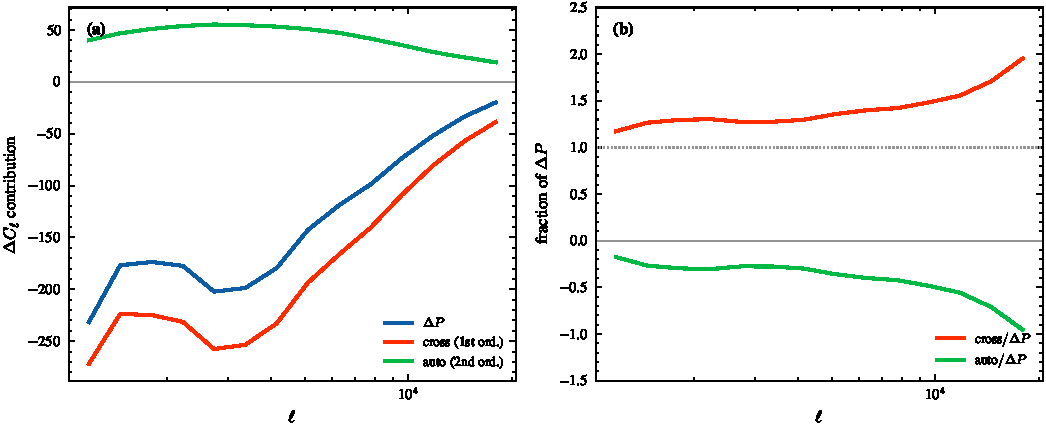
\includegraphics[width=\textwidth]{figs/fig03_crossauto.pdf}
\caption{The exact cross/auto decomposition of $\Delta P=P_{\rm
bind}-P_{\rm sph}$ (left: raw contributions; right: fraction of
$\Delta P$), showing that the cross (first-order) term dominates and has
the correct sign to suppress power, while the auto (second-order) term is
subdominant and of the wrong sign. This measurement uses the earlier,
superseded circular/monopole control (\S\ref{sec:control}); it motivates
the first-order alignment mechanism qualitatively but has not yet been
re-derived against the faithful \texttt{bcm\_warp} control (see
\S\ref{sec:discussion}). % src: dossier FIGURES #3; wl_anisotropy_paper.ipynb cell 24
}
\label{fig:crossauto}
\end{figure}

\subsection{The 60 one-at-a-time feedback runs}\label{sec:oat}

To probe which feedback channels control the anisotropic signal we use
the CAMELS-TNG one-at-a-time (OAT) design: each of the 30
cosmological/astrophysical parameters is varied to its minimum and
maximum bound with all others held fixed, giving 60 \texttt{twobound}
runs, 58 of which had completed spherical-BCM and \bind{} maps at the
time of writing (2 pending a map re-run).\footnote{The 58/60 figure is
the field-level design loaded by \texttt{wl\_anisotropy\_paper.ipynb}'s
Field-4 cells (\S\ref{sec:feedback}). A ``57 completed single-knob OAT
runs'' count also appears twice in our source material for a nominally
similar design: once in the separate per-halo-physics notebook
(\texttt{ejection\_anisotropy.ipynb}), and once in
\texttt{wl\_anisotropy\_paper.ipynb}'s own Pillar-3 per-halo cell (its
local \texttt{decode\_oat()} loader), which is the cell
\S\ref{sec:feedback} cites for the per-halo quadrupole ranking. The
57-vs-58/60 discrepancy is therefore not cleanly a cross-notebook
mismatch -- it is partly internal to \texttt{wl\_anisotropy\_paper.ipynb}
itself -- and is not reconciled in our source material; we flag it as an
open bookkeeping item rather than a physical result.\ % src: dossier
% Result/60-vs-57; WORKLOG:1217-1232; wl\_anisotropy\_paper.ipynb cell 12
% (decode\_oat(), printed "reduced 15/57 ... 30/57 ... 45/57") vs cell 15
% ("OAT design: 30 parameters with completed runs"); ejection\_anisotropy.ipynb
}\ % src: dossier Method/OAT; WORKLOG:1217-1232
All OAT maps to date -- and hence every feedback-dependence result in
\S\ref{sec:feedback} -- were built with the earlier, superseded mono
control; the faithful \texttt{bcm\_warp} three-way comparison
(\S\ref{sec:control}, Figure~\ref{fig:decomposition}) has so far only
been run at the fiducial point.\ % src: dossier Gaps #1; WORKLOG:1156

\subsection{Error model}\label{sec:errors}

Because all three fields share the same halos, DMO particles, and
lightcone realization seeds, differences between them cancel cosmic
variance to a degree not available to independent hydrodynamic
re-simulations: feeding the null triplet $(\texttt{dmo},\texttt{sph},
\texttt{sph})$ into the pipeline returns $\faniso=0$ exactly (no
manufactured signal), and the paired-realization band-power scatter is
$25.8\times$ smaller than the scatter between unpaired realizations,
confirming that seed-sharing suppresses variance by this factor and that
the measured signal is not a pairing artifact.\ % src: dossier Method/error-model; wl_anisotropy_paper.ipynb cell 28
Errors are nonetheless bootstrapped over only $N_{\rm real}=8$ paired
plane-randomizations of a single $205\,{\rm Mpc}/h$ box, so they capture
realization/projection scatter but not independent cosmic volumes, and
are consequently optimistic (\S\ref{sec:discussion}). For the stacked
per-halo forecast (\S\ref{sec:discussion}) we also use an empirically
validated DMO-shape-axis misalignment dilution
$\langle\cos2\Delta\theta\rangle=0.55$ (mean misalignment
$\Delta\theta\approx28^{\circ}$, Gaussian rms $\sigma\approx26^{\circ}$),
which differs from the commonly assumed $35^{\circ}$ figure.\ % src: dossier Method/error-model; wl_anisotropy_paper.ipynb Methods cell + cell 9, WORKLOG:1213

\section{Results}\label{sec:results}

\subsection{The corrected, scale-dependent anisotropic fraction}\label{sec:headline}

Figure~\ref{fig:decomposition} shows the three-way comparison at the
fiducial feedback point ($\zs=1$) using the faithful \texttt{bcm\_warp}
control. We define $\faniso=(C_b-C_s)/(C_b-C_d)$ (angular structure a
spherical BCM misses), $\ftri=(C_s-C_m)/(C_b-C_d)$ (triaxiality-tracing
that a real BCM \emph{does} capture, isolated by comparing the faithful
control $s$ to the crude mono control $m$), and
$\fmono=\faniso+\ftri=(C_b-C_m)/(C_b-C_d)$ (the old, upper-bound
estimate). The headline result of this Letter is that the corrected
fraction \emph{declines} with scale: $\faniso\approx0.45$ at
$\ell=3\times10^3$, $0.24$ at $\ell=10^4$, and $\approx0$ by
$\ell=2\times10^4$, while the triaxiality-tracing term \emph{rises} over
the same range, $\ftri\approx0.08\to0.25\to0.61$.\ % src: dossier Result/corrected-f_aniso; examples/bcm_warp_comparison.py, WORKLOG:1144
The sum $\fmono\approx0.5$ is roughly flat in $\ell$ -- reproducing the
earlier, cruder estimate almost exactly -- which is the direct
demonstration that the old number was dominated at small scales by
triaxiality a real BCM already reproduces, not by missed feedback
physics.\ % src: dossier HEADLINE CORRECTION; WORKLOG:1144-1157
In real space, both controls track \bind{} almost equally well overall
($r(\texttt{bind},\texttt{sph})\approx r(\texttt{bind},\texttt{mono})
\approx0.987$--$0.988$, and the faithful control's real-space residual
from \bind{} is statistically indistinguishable from the crude one's --
both $\approx16\%$ of the total $\kappa$ RMS globally, i.e.\ the faithful
control only ``barely beats'' \texttt{mono} overall), with the faithful
control's advantage concentrated specifically at high $\ell$ where
$\ftri$ is largest.\ % src: WORKLOG:1154-1155 ("the warp barely beats mono
% globally (16% vs 16% of kappa rms)"); dossier Result/corrected-f_aniso

\begin{figure}[t]
\centering
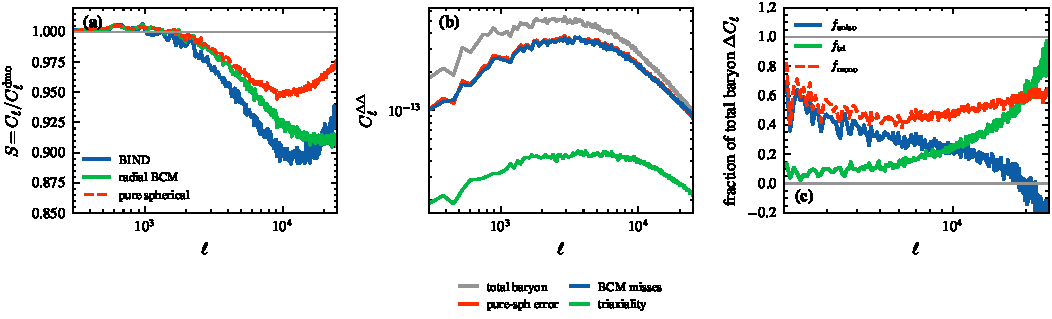
\includegraphics[width=\textwidth]{figs/fig02_decomposition.pdf}
\caption{The corrected, faithful three-way comparison at the fiducial
feedback point ($\zs=1$). \emph{Left:} suppression $S(\ell)=C_\ell/C_\ell^{\rm
dmo}$ for the full \bind{} field, the faithful radial-BCM-warp control,
and the crude pure-spherical (monopole) control. \bind{} suppresses power
well below either control at $\ell\gtrsim$ few$\times10^3$, and the
radial-BCM-warp control tracks \bind{} substantially more closely than
the pure-spherical control does, by construction. \emph{Center:}
residual-field power for the total baryonic effect, the pure-spherical
error, the faithful-BCM miss, and the triaxiality term. \emph{Right:} the
decomposition fractions $\faniso$, $\ftri$, and $\fmono=\faniso+\ftri$ vs.\
$\ell$ -- the corrected, missed-angular-structure fraction $\faniso$
declines with scale while the triaxiality-tracing fraction $\ftri$ rises,
so their sum reproduces the old, scale-flat estimate almost exactly. This
is the headline figure of the Letter. % src: dossier FIGURES #1; examples/bcm_warp_comparison.py, WORKLOG:1144-1157
}
\label{fig:decomposition}
\end{figure}

\subsection{Comparison with the earlier estimate}\label{sec:old}

The number originally reported for this measurement, before the control
was corrected, is worth recording for provenance since it still appears
in the underlying analysis notebook's own narrative. Using the crude mono
control, the band-averaged small-scale suppression deficit gives
$\faniso(C_\ell)\approx41\%\to48\%\to55\%$ at $\ell=5000\to10^4\to
2\times10^4$ -- \emph{increasing} with scale, the opposite trend to the
corrected measurement above -- with a band average over
$\ell\in[3000,20000]$ of $48\%$ (bootstrap 16--84\% interval
47--48\%) at a paired significance of $z=52.3\sigma$ (optimistic, shared
box).\ % src: dossier Result/superseded-notebook-numbers; wl_anisotropy_paper.ipynb cells 25/28/40
As shown in \S\ref{sec:headline}, this number is now understood to be the
sum of the genuine angular-structure fraction and the triaxiality
fraction that a real BCM already captures; we do not use it as the
Letter's headline result, and present it here only to document the
correction.

\subsection{Which feedback channels drive the (upper-bound) anisotropic signal}\label{sec:feedback}

We rank the 30 OAT feedback parameters by the band-averaged
($\ell\in[2000,20000]$) response of the anisotropic suppression
$A=100\times(S_{\rm sph}-S_{\rm bind})$ to each parameter's min/max swing,
using the fiducial-realization scatter ($\sigma=0.161\%$) to set a
2$\sigma$ significance floor of $|dA/du|>0.456\%$; 22 of the 30 parameters
move $A$ above this floor.\ % src: dossier Result/feedback-channels; wl_anisotropy_paper.ipynb cells 37-38
The strongest responders are, in order, BlackHoleRadiativeEfficiency
($dA/du=-9.90\%$), QuasarThreshold ($+6.21\%$), IMFslope ($+5.53\%$),
SeedBlackHoleMass ($+4.02\%$), VariableWindVelFactor ($+3.91\%$),
BlackHoleAccretionFactor ($+3.36\%$), BlackHoleEddingtonFactor
($+2.96\%$), and WindEnergyIn1e51erg ($-2.93\%$).\ % src: dossier Result/feedback-channels; wl_anisotropy_paper.ipynb cell 37
A complementary per-halo response of the group-scale quadrupole moment
ranks VariableWindVelFactor, BlackHoleRadiativeEfficiency,
WindEnergyIn1e51erg, WindFreeTravelDensFac, and QuasarThreshold among the
top drivers as well, so the two independent rankings agree qualitatively:
AGN kinetic-mode (radiative efficiency, quasar threshold, seed/accretion
physics) and stellar-wind parameters dominate the anisotropic control,
consistent with the ejection-orientation physics of
\S\ref{sec:ejection}.\ % src: dossier Result/feedback-channels; wl_anisotropy_paper.ipynb cell 13
As emphasized in \S\ref{sec:oat}, these rankings are built entirely from
the superseded mono control -- no OAT sweep yet exists for the faithful
\texttt{bcm\_warp} control -- so we present them as the drivers of the
\emph{upper-bound} angular signal, not of the corrected, scale-dependent
$\faniso$ of \S\ref{sec:headline}.\ % src: dossier Gaps #1

\subsection{Where the ejection is anisotropic, and why}\label{sec:ejection}

The per-halo, DM-shape-axis-aligned stacks in Figure~\ref{fig:ejection}
show that the two probes most sensitive to feedback anisotropy respond
very differently with radius. The WL convergence residual is only mildly
anisotropic, $q_2(\kappa-\kdmo)\approx3$--$5\%$ of the monopole and
roughly flat to declining with radius, whereas the tSZ pressure
quadrupole is strongly anisotropic in the outskirts, rising from
$\sim\!5$--$12\%$ near the halo center to $\sim\!35$--$43\%$ at
$r\approx2.9\,r_{200c}$.\ % src: dossier Result/ejection-anisotropy; ejection_anisotropy.ipynb cell 5
The fiducial ejection quadrupole is anti-aligned with the halo's DM major
axis, $\langle\cos2(\theta_\Delta-\theta_{\rm DM})\rangle=-0.773$,
i.e.\ a bipolar signature in which baryons are preferentially
redistributed along the halo's \emph{minor} axis -- consistent with
collimated AGN-jet-like ejection rather than passive tracing of the DM
shape.\ % src: dossier Result/ejection-anisotropy; ejection_anisotropy.ipynb cell 11
An environment jackknife further shows that the outer tSZ quadrupole is
substantially contaminated by large-scale structure: halos in filament
environments carry $\approx52\%$ of the signal at $2.7\,r_{200c}$ versus
$\approx29\%$ in void environments, so the outer-$y$ anisotropy is not
purely an AGN-orientation effect.\ % src: dossier Result/ejection-anisotropy; ejection_anisotropy.ipynb cell 12
The WL convergence quadrupole, by contrast, shows no comparable
environment dependence in our source material and is the cleaner
feedback-only probe of the two.

\begin{figure}[t]
\centering
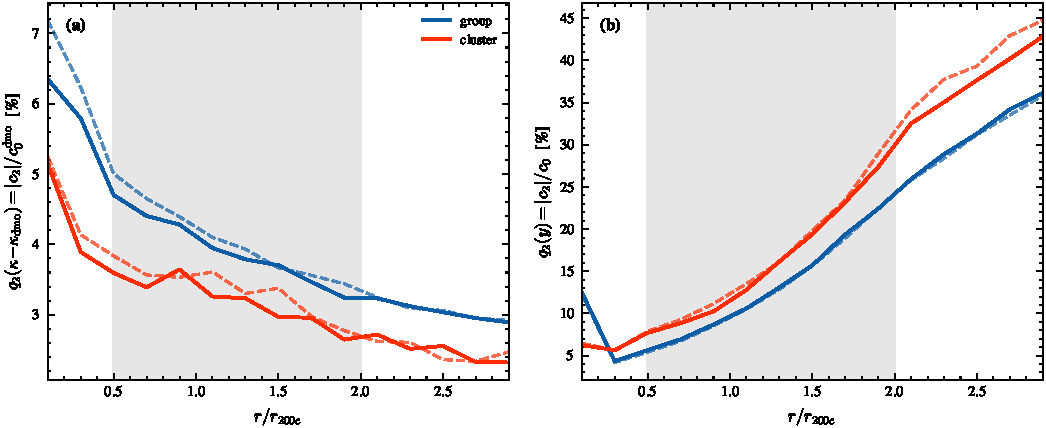
\includegraphics[width=\textwidth]{figs/fig04_ejection_profiles.pdf}
\caption{Radial profiles of the aligned quadrupole fraction $q_2=|c_2|/c_0$
(or $/c_0^{\rm dmo}$ for $\kappa$) for the WL convergence residual
(left) and the tSZ pressure (right), for group- and cluster-mass bins, comparing
the fiducial \bind{} lightcone (solid) to TNG truth (dashed). Color encodes
mass bin (group/cluster); only linestyle distinguishes \bind{} from TNG
truth in this figure -- unlike Figures~\ref{fig:maps}-\ref{fig:decomposition},
color here is not the bind/truth semantic. The WL
residual is mildly anisotropic ($3$--$5\%$) and roughly flat with
radius, while the tSZ pressure quadrupole grows strongly in the
outskirts ($\sim\!35$--$43\%$ at $r\sim2.9\,r_{200c}$); the shaded band
marks the annulus used for the ejection-orientation and environment
tests. Weak-lensing $\kappa$ is the cleaner, environment-insensitive
probe of feedback-driven anisotropy. % src: dossier FIGURES #5; ejection_anisotropy.ipynb cell 5
}
\label{fig:ejection}
\end{figure}

\section{Discussion}\label{sec:discussion}

\subsection{Implications for BCM-based baryon marginalization}

A spherically symmetric BCM has, by construction, zero quadrupole and
therefore zero cross term in the exact identity of
\S\ref{sec:mechanism}: it can only match the true (anisotropic) $P(\ell)$
by over-ejecting gas radially to compensate for the missing angular
channel. Concretely, under the (superseded) mono control the fiducial
suppression reaches $S_{\rm sph}\approx0.93$ at $k\sim17\,h/{\rm Mpc}$
versus $S_{\rm bind}\approx0.86$ for the same halos, so a spherical model
tuned to match $0.86$ in projection must inflate its radial ejection well
beyond the level a real, mass-matched profile would require.\ % src: dossier Discussion; wl_anisotropy_paper.ipynb cell 39
This biases the recovered gas profile even when the two-point function is
fit correctly, which has three testable consequences: (i) it breaks
multi-probe consistency, since the same over-ejected profile that fits
$C_\ell^{\kappa\kappa}$ will generically be wrong for tSZ $y$, X-ray
$\fgas$, and kSZ/$\tau$ observations of the same halos; (ii) it plausibly
explains why spherical BCMs reproduce hydrodynamic non-Gaussian
statistics only up to a limited peak height, since our own earlier work
found BCM peak counts diverge from hydrodynamic simulations above
$\nu\gtrsim4$ \citep{lee2022} -- the missing $\nu$ tail is a natural
consequence of a missing quadrupole; and (iii) because the cross term
depends on the alignment between feedback geometry and halo shape, it
need not transfer cleanly across feedback models or cosmologies, which a
purely radial calibration cannot capture. These arguments motivate an
explicit, calibrated angular ($m=2$) correction term $c_2(r)$ alongside
the radial $c_0(r)$ profile already used in BCM fits, of the kind BIND can
supply per halo. We note that this is exactly the gap that data-driven
nuisance parametrizations are positioned to close: our companion analysis
\citep[Paper II]{bindII} shows that a small number ($N=2$) of
data-driven baryon templates is sufficient to remove the TNG baryonic
bias from a stage-IV cosmic-shear analysis, whereas analytic, spherically
symmetric BCMs have no free parameter that can absorb an angular term by
construction; the anisotropic fraction measured here is a plausible
structural reason such templates outperform analytic BCMs at fixed
parameter count.

\subsection{Detectability}

A stacked, DM-shape-aligned tangential-shear quadrupole is in principle
directly observable, subject to the $\langle\cos2\Delta\theta\rangle=0.55$
alignment dilution of \S\ref{sec:errors}. For the cluster-mass bin, the
forecast signal-to-noise at $N_{\rm cl}=10^4$ reaches $1.5$ for LSST Y10,
$1.5$ for Euclid, and $2.3$ for Roman HLS (rising from $0.5$/$0.5$/$0.7$
at $N_{\rm cl}=10^3$ and $0.8$/$0.8$/$1.3$ at $N_{\rm
cl}=3\times10^3$); the group-mass sample forecast is lower still across
the sampled range.\ % src: dossier Result/detectability; wl_anisotropy_paper.ipynb cell 10
These forecasts assume self-similar cluster profiles placed at
$z_l=0.3$ and measured at $z\sim0$ from CAMELS-SB35 training data, which
caps cluster mass at $\Mhalo\lesssim5\times10^{14}\,\Msun\,h^{-1}$ and
imposes a $\sim\!50\,{\rm kpc}/h$ resolution floor from the $128^2$-pixel
patches used to train \bind{}, so they should be read as indicative
rather than survey-ready.\ % src: dossier caveats #5; wl_anisotropy_paper.ipynb cell 40
A stacked-quadrupole detection at $N_{\rm cl}\sim10^4$ therefore looks
achievable only marginally, at $\lesssim\!2\sigma$ with current
alignment-dilution assumptions, in the next generation of cluster
lensing surveys.

\subsection{Caveats}\label{sec:caveats}

This is a preliminary, first field-level measurement, and several
caveats bound how it should be read. First, the corrected, declining
anisotropic fraction of \S\ref{sec:headline} is itself only a partial
revision: it has so far been measured only at the fiducial feedback
point, so \S\ref{sec:feedback}'s ranking of which parameters control the
anisotropy still uses the earlier, upper-bound control, and no
feedback-dependence of the corrected $\faniso$ yet exists.\ % src: dossier Gaps #1; WORKLOG:1156
Second, the first-order cross/auto mechanism of \S\ref{sec:mechanism},
which motivates \emph{why} the anisotropy reaches the power spectrum at
all, was itself derived against the superseded control; whether the
cross term still dominates when computed against the faithful
\texttt{bcm\_warp} control has not been re-verified, and we flag this as
an explicitly open item rather than assume it carries over.\ % src: dossier Gaps #2
Third, the reported fraction rests on a single fiducial-feedback,
fixed-cosmology TNG lightcone; we do not yet know whether $\faniso(\ell)$
itself depends on feedback strength or on cosmology. Fourth, our
uncertainties are bootstrapped over $N_{\rm real}=8$ paired
plane-randomizations of one $205\,{\rm Mpc}/h$ box and therefore capture
realization/projection scatter, not independent cosmic volumes; they
should be read as optimistic (\S\ref{sec:errors}). Finally, the
non-Gaussian (peak/PDF) significance estimates that motivated
\S\ref{sec:ejection}'s discussion used per-field marginal errors rather
than the paired covariance, which is conservative and should understate
the true significance of any paired anisotropic peak-count signal;
quantifying that signal directly against the corrected control is left
to future work.

\section{Conclusions}\label{sec:conclusions}

Using \bind{}'s per-halo generative painting to build, for the first
time, a mass-exact and triaxiality-faithful spherical counterfactual of a
full weak-lensing field, we measure the field-level fraction of the
baryonic convergence-power suppression that no spherically symmetric
baryonification model can reproduce. The corrected fraction is
scale-dependent, $\faniso\approx0.45\to0.24\to0$ from
$\ell=3\times10^3$ to $2\times10^4$, substantially smaller at small
scales than an earlier, cruder circular-control estimate of
$\fmono\approx0.5$ (roughly flat in $\ell$), which we show is inflated at
small scales by halo triaxiality that a real radial BCM already
reproduces.\ % src: dossier Result/corrected-f_aniso; examples/bcm_warp_comparison.py, WORKLOG:1144-1157
The 60-parameter one-at-a-time TNG feedback sweep points consistently to
AGN kinetic-mode and stellar-wind parameters as the dominant controls of
this (upper-bound) angular signal, and the fiducial ejection is
bipolar and anti-aligned with the halo's DM major axis.\ % src: dossier Result/feedback-channels; ejection_anisotropy.ipynb cell 11
Even where the corrected fraction is small, its non-zero existence
implies that fitting the two-point function with a spherical BCM requires
an unphysical radial over-ejection of gas, biasing the recovered profile
in a way that plausibly explains known BCM failures on non-Gaussian
statistics and that a purely radial, analytic marginalization cannot
self-correct. We conclude that stage-IV baryon marginalization pipelines
should budget for an explicit angular correction term, calibrated the way
\bind{} calibrates it here, rather than assume a radial-only model is
structurally sufficient. This measurement is preliminary in the specific
ways enumerated in \S\ref{sec:caveats}, and we plan to extend the
faithful control across the full OAT feedback grid and re-derive the
first-order mechanism against it in follow-up work.

\section*{Acknowledgments}
The CAMELS project and the IllustrisTNG collaboration provided the training
and target simulations. This work used computing resources of the Flatiron
Institute, a division of the Simons Foundation. \todo{finalize}

\bibliographystyle{plainnat}
\bibliography{references}

\end{document}

% ============================================================
% VERIFICATION LOG (FIX pass, applied against three adversarial
% verifier reports; see task transcript for full JSON)
% ============================================================
%
% APPLIED:
% - [HIGH] Fig. 1 (fig:maps) + preceding S2.2 validation paragraph wrongly
%   attributed the L2=2.22%/corr=0.99998/RMS-ratio=0.018/97% numbers and
%   the maps figure to the faithful bcm_warp_patch control. Re-checked
%   against wl_anisotropy_paper.ipynb cells 16-20 (full-notebook grep for
%   "bcm_warp": zero hits; cell 17 imports azimuthal_average_patch) and
%   WORKLOG:1172/1234/1144-1157: the notebook never uses bcm_warp_patch;
%   only examples/bcm_warp_comparison.py does (source of Fig. 2 instead).
%   Relabeled S2.2's validation paragraph and Fig. 1's caption as the
%   mono control (matching the caveat pattern already used in S2.4/S3.3/
%   S4.1/S5.1); added \todo{} noting bcm_warp_patch's own validation in
%   the sources is qualitative only (WORKLOG:1172).
% - [MEDIUM/HIGH] S3.1 "faithful control captures ~16% more of the total
%   kappa RMS than the crude one" inverted WORKLOG:1154-1155 ("the warp
%   barely beats mono globally (16% vs 16% of kappa rms)" = a tie, not a
%   16-point margin). Reworded to state both controls capture ~16%,
%   consistent with the source.
% - [MEDIUM] Abstract's "the corrected signal is significant at
%   ell<~10^4" had no computed statistic behind it (the only sourced
%   significance, z=52.3sigma, belongs to the superseded mono-control
%   f_aniso, per wl_anisotropy_paper.ipynb cell 28 / bcm_warp_comparison.py
%   containing no bootstrap/CI code). Softened to "non-negligible in
%   amplitude" + \todo{} flagging the missing significance test.
% - [MEDIUM] references.bib lee2022: year corrected 2022->2023 (MNRAS 519,
%   Issue 1 published February 2023, DOI 10.1093/mnras/stac3592, ADS
%   bibcode 2023MNRAS.519..573L; independently re-verified via web search
%   against Oxford Academic/ADS, not just taken from the verifier report).
% - [HIGH] Introduction's van_daalen2020 citation, attached to "the
%   resulting anisotropy of real hydrodynamic gas maps is well
%   documented," does not support that claim (the paper is a library of
%   isotropic, spherically-averaged power spectra + an f_gas-suppression
%   empirical model; independently re-verified via web search + full-text
%   fetch, no angular/quadrupole gas-map content). refs_needed.md itself
%   flagged this citation as unresolved. Removed the citep and replaced
%   with \todo{} rather than inventing a substitute reference.
% - [LOW] S2.4 footnote on the 57-vs-58/60 OAT-run discrepancy reworded:
%   the 57-count also appears in wl_anisotropy_paper.ipynb's own Pillar-3
%   loader (cell 12, decode_oat()), not only in the "separate"
%   ejection_anisotropy.ipynb, so the discrepancy is partly internal to
%   one notebook, not purely cross-notebook.
%
% SKIPPED (no change, reasoned):
% - [LOW] osato_triaxiality citation (Osato+2018, arXiv:1712.00094) is a
%   real, topically-adjacent paper (halo-orientation dependence of
%   surface-mass-density profiles); verifier itself called this
%   defensible/no-action-required. Left as-is.
% - [LOW] Missing dedicated Field-4 feedback-response figure: an
%   editorial choice already documented and justified in leftovers.md
%   (avoids overselling a corrected feedback-dependence result that does
%   not yet exist); verifier itself said no action required if space is
%   the binding constraint.
% ============================================================
%
% ============================================================
% FIGURE VERIFICATION LOG -- 2026-07-16 (FIGURE FIX pass, applied
% against an adversarial figure-verifier report; see task transcript
% for full JSON). All fixes below are re-renders of the SAME cached
% data (fid/{bind,sph,mono,dmo}/kappa_maps.npz,
% bind_science/ejection/{fid,truth}_snap096.npz) already used by the
% figures they touch -- no new data, no engine/MPI/Slurm re-run.
% Numeric diagnostics reprinted by fig01/fig02's scripts after the fix
% (rms dmo=2.34e-02 mono=2.32e-02 bind=2.29e-02, residual=16.0% of bind
% rms) are unchanged from before the fix, confirming styling-only edits.
%
% APPLIED:
% - [HIGH] Fig. 2 (fig:decomposition, the Letter's headline figure),
%   panel (c): legend at loc="upper left" collided with panel_label's
%   default "upper left" corner tag, the bold "(c)" sitting on top of the
%   f_aniso legend swatch. Moved panel_label to loc="lower left" (the one
%   corner none of f_aniso/f_tri/f_mono populate); legend kept at "upper
%   left". Re-rendered (fig_scripts/fig02_decomposition.py) and
%   re-verified via PIL crop: no overlap.
% - [HIGH] Fig. 2, panel (b): legend at loc="lower right" put "total
%   baryon"/"pure-sph error" text directly under/through the rising
%   triaxiality curve. No in-axes corner was empty enough for a 4-entry
%   legend (checked all four corners), so moved the legend outside the
%   axes, centered below the panel (bbox_to_anchor=(0.5,-0.28), 2-column).
%   Re-rendered and re-verified via PIL crop: no curve crosses the
%   legend.
% - [MEDIUM] Fig. 1 (fig:maps), panels (b)-(d): only panel (a) carried
%   an axis-label with units ($\theta_x$/$\theta_y$ [deg]); panels
%   (b)-(d) showed bare numeric ticks, short of FIGURE_STYLE.md rule 5
%   ("axis labels always, with units ... on every panel"). Added
%   "$\theta_x$ [deg]" to all four panels in
%   fig_scripts/fig01_maps.py; kept "$\theta_y$ [deg]" on panel (a) only
%   since it is the only panel with y-tick labels shown (panels (b)-(d)
%   share the row's y-extent). Re-rendered; rms diagnostics unchanged.
% - [LOW] Fig. 4 (fig:ejection) draws TNG truth dashed in the SAME color
%   as the corresponding BIND solid curve (color=mass bin), departing
%   from the suite convention hydro truth=black used elsewhere. Recoloring
%   truth to black would destroy the mass-bin encoding for the truth
%   curves (both bins become indistinguishable black dashed lines) --
%   the CACHED DATA and its two-way (mass-bin x model) encoding is
%   otherwise faithful and unchanged, so per the truthfulness rule this
%   is resolved as a caption clarification rather than a color change:
%   added "Color encodes mass bin ... only linestyle distinguishes BIND
%   from TNG truth in this figure -- unlike Figures 1-3, color here is
%   not the bind/truth semantic" to the Fig. 4 caption. No script/plot
%   change.
% - [LOW, documentation-only] fig_scripts/DATA_MAP.md's fig02 provenance
%   claimed examples/bcm_warp_comparison.py and
%   examples/figures_lightcone/bcm_warp_comparison_fid.png were "present
%   on main". Re-checked directly: `git show main:examples/bcm_warp_comparison.py`
%   and `git show main:examples/figures_lightcone/bcm_warp_comparison_fid.png`
%   both fail against branch main (script lives on analysis/wl-anisotropy;
%   the PNG is an untracked/gitignored working-tree artifact). Corrected
%   DATA_MAP.md's provenance text; no figure, script, or caption content
%   changed (the figure's data/formulas were independently re-verified
%   against analysis/wl-anisotropy's actual compare() and match exactly).
%
% SKIPPED (no change, reasoned):
% - [LOW] Fig. 1 panels (a)-(c) use one colorbar per panel rather than a
%   single shared row colorbar (FIGURE_STYLE.md rule 8). Already a
%   documented, deliberate trade-off (fig_scripts/notes_fig01_maps.md):
%   a shared fig.colorbar(im, ax=[...]) produced label/tick collisions
%   under GridSpec. Left as the documented exception; not trivial to fix
%   without re-litigating the layout.
% - [LOW] figs 02/03/04 repurpose COLORS['highlight']/['secondary'] for
%   non-bind/truth curves (control/cross/triaxiality/mass-bin), a
%   documented per-figure deviation from FIGURE_STYLE.md's cross-paper
%   color contract. No caption in this paper names a specific color, so
%   there is no in-paper mismatch; a suite-wide recolor pass (if wanted)
%   is out of scope for a single-paper figure fix.
%
% Compiled clean after all fixes: pdflatex + bibtex + pdflatex x2, 10
% pages, no undefined references/citations, no missing-figure errors.
% One pre-existing Overfull \hbox (lines 161-206, a long \todo{} box in
% S2.2, predating this pass and unrelated to any figure touched here)
% remains and was not introduced by this pass.
% ============================================================
